%\usepackage [ISO-8859-1]{inputenc}
\documentclass[a4paper,12pt,oneside]{amsbook}
\usepackage[T1]{fontenc}
\usepackage{listings}
\usepackage{textcomp}
\usepackage{multicol,calc}
%\usepackage{euler}
%\usepackage{garamond}
\usepackage{hyperref}

\usepackage{newcent}
%\fontfamily{fxm}\selectfont
\usepackage{fancyhdr}
\pagestyle{fancy}
% Detta paket skoter grafiken
%\usepackage[dvips]{graphicx}
\usepackage[pdftex]{graphicx}

\usepackage{amsthm}
\usepackage{amsmath}
\usepackage[swedish]{babel}
% For bortkommentering
\usepackage{verbatim}
% For att slippa indentering av Sections och SubSections
\usepackage{indentfirst}

% Har stalls paragrafindentering och avstand mellan stycken och rader mm
\setlength{\parindent}{0pt}
\setlength{\parskip}{6pt}
\setlength{\baselineskip}{12pt}
% Har definieras sidan
\setlength{\voffset}{-15mm}
\setlength{\hoffset}{-5.5mm}

\setlength{\topmargin}{0mm}
\setlength{\headheight}{10mm}
\setlength{\headsep}{8mm}
\setlength{\footskip}{16mm}

\setlength{\evensidemargin}{0mm}
\setlength{\oddsidemargin}{0mm}

\setlength{\marginparsep}{0mm}
\setlength{\marginparwidth}{0mm}

\setlength{\textwidth}{170mm}
\setlength{\textheight}{230mm}
\setlength{\paperwidth}{210mm}
\setlength{\paperheight}{297mm}
\setlength{\headwidth}{170mm}
% Huvud och Fot
%\fancypagestyle{}{
\fancyhf{}\fancyhead[c]{\small{\textit{Programmeringsolympiaden Kvalificering 2023}}}
\fancyfoot[c]{\thepage}
\renewcommand{\headrulewidth}{0.4pt}
\renewcommand{\footrulewidth}{0.4pt}
\newenvironment{lista}
{\begin{itemize}
\setlength{\parindent}{0pt}
\setlength{\itemsep}{6pt}}
{\end{itemize}}
% Uppgifter
\newcounter{probnr}
\newenvironment{tal}{%
\begin{list}
%{\textbf{\arabic{section}.\arabic{probnr}}} {\usecounter{probnr}
{\textbf{\arabic{probnr}}} {\usecounter{probnr}
\setlength{\leftmargin}{0mm}
\setlength{\rightmargin}{0mm}
\setlength{\labelwidth}{-1mm}
\setlength{\labelsep}{1mm}}
\setlength{\itemsep}{6pt}
}{\end{list}}
% Definition av avsnitt: FAKTA, EXEMPEL, PASTAENDE
\newtheorem{fakta}{Fakta}
\newtheorem{exempel}{Exempel}
\newtheorem{problem}{Problem}
%
\newtheoremstyle{test}% NAME
{20pt}      % ABOVESPACE
{10pt}      % BELOWSPACE
{\sffamily} % BODYFONT
{0pt}       % INDENT
{\scshape}  % HEADFONT
{}          % HEADPUNCT
{\newline}  % HEADSPACE
{}          % CUSTOM-HEAD-SPEC

\theoremstyle{test}
\newtheorem{program}{Program}
\newcommand{\sv}[1]{\textsc{#1}}            % Sma versaler
\newcommand{\fe}[1]{\textbf{#1}}            % FET
\newcommand{\ku}[1]{\textit{#1}}            % KURSIV
\newcommand{\cu}[1]{\texttt{#1}}            % Courier
\newcommand{\sk}[1]{\texttt{#1}}            % Courier
\newcommand{\rubrik}[1]{\begin{center}\sf\huge{#1}\normalsize\rm\end{center}}
\begin{document}
%\DeclareGraphicsExtensions{.jpg,.pdf,.mps,.png,.eps}



\thispagestyle{fancy}
\lstset{basicstyle=\ttfamily,
  breaklines=true}
% ----------------------------------------------------

\begin{center}
\Huge{Programmeringsolympiaden 2023}
\end{center}
\vspace{-1.2cm} 
\specialsection*{Tävlingsregler för skolkvalet}
\begin{lista}
\item Tävlingen äger rum på av skolan bestämt datum under {\bf fyra
    timmar. Ingen förlängning ges för lunch eller raster.} Eleven ska i förväg komma överens med läraren om att använda egen dator eller en som skolan tillhandahåller. I vilket fall som helst måste eleven befinna sig i avtalad lokal på skolan. {\bf På grund av pandemin kan i undantagsfall tävling ske från annan plats godkänd av läraren, givet tillräcklig övervakning.}
\item Tävlingen består av sex uppgifter som vardera ska lösas genom ett
  datorprogram i valfritt programmeringsspråk.
\item {\bf Indata kan läsas in i programmet på valfritt sätt}, t.ex. genom att programmet för en dialog med användaren (som i körningsexemplena i uppgifterna), att de skrivs in i ett grafiskt gränssnitt eller att datafiler skickas till {\em standard input}. Kom bara överens med din lärare om hur programmet ska testas.
\item Dina lösningar kommer att testköras med förpreparerade
  indata. Varje uppgift testas normalt med 5 testfall, som vardera ger
  1 poäng om ditt program skriver ut korrekt svar inom en exekveringstidsgräns av
  {\bf 3 sekunder}. Ingen test av indata behöver göras, den följer specifikationerna 
i uppgiften.
\item Det är ofta olika begränsningar på de olika testfallen, t.ex.\ storleken på
indata eller andra inskränkningar. Detta anges i uppgiften. {\bf Observera att det kan vara
helt olika svårighetsgrad på en uppgift beroende på dessa skillnader. Det kan därför vara
lättare att få delpoäng på en uppgift som verkar svår än att få full
poäng på en uppgift som verkar lättare.} Informationen om delpoäng är
därför extremt viktig för att planera sin
tävling.
\item Rättningen utförs på samma eller likvärdig dator. Ändringar
  i källkoden tillåts ej efter tävlingen. Om programmet
  inte kan kompileras ges 0 p.\ på uppgiften. 
\item Om något av följande inträffar ger
  det {\em testfallet} 0 poäng, men programmet fortsätter testas med övriga testfall.
\begin{lista}
\item Exekveringstiden överstiger 3 sekunder \vspace{-0.2cm}
\item Exekveringsfel (run time error) \vspace{-0.2cm}
\item Fel svar \vspace{-0.2cm}
\end{lista}

\item Deltagandet är individuellt vilket bland annat innebär att inget utbyte av idéer eller 
filer får ske under tävlingen.  
\item Hjälpmedel: Valfritt skriftligt material, material som finns installerat på datorn samt material som finns tillgängligt på internet. Det är \ku{inte} tillåtet att aktivt kommunicera på internet (t.ex. chatta eller ställa frågor till ett forum) utan endast att söka efter information. Räknedosa är tillåten.
\item Tävlingsbidraget ska lämnas in i form av källkodsfiler (uppg1...uppg6 med passande filtillägg) som läggs på överenskommen plats. Ingen hänsyn tas till andra filer. Var noga 
med att lämna in den korrekta versionen av ditt program.  
\end{lista}

%De högst placerade i kvalet går vidare till finalen där landslagsplatser till BOI i Sverige och IOI i Japan står på spel.
\begin{center}
\Large Lycka till!
\end{center}
%\end{document}

\newpage
\specialsection*{Uppgift 1 -- Morötter}

Tor och hans mor älskar morötter. Varje dag ställer de fram en skål med 40 morötter och äter sedan morötter oavbrutet tills skålen är tom. Om de båda är redo att ta en morot när det bara finns en kvar, så tar ingen av dem den sista.

Skriv ett program som, givet antal sekunder det tar för Tor respektive hans mor att äta varje morot (båda heltal), beräknar hur många morötter var och en får.

\begin{center}
  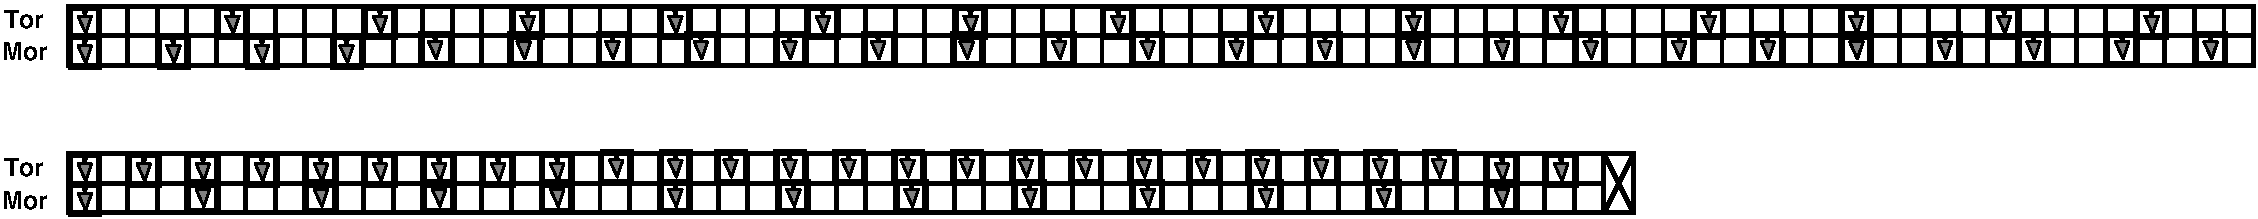
\includegraphics[width=17cm]{morot.pdf}
\end{center}
\ku{Tidsschema för morotsätningen i exempel 1 (överst) och exempel 2 (underst). I det andra exemplet kommer ingen att ta den sista moroten.}

\fe{Körningsexempel 1}
\begin{verbatim}
Tors tid ? 5
Mors tid ? 3

Svar: Tor 15,   Mor 25
\end{verbatim}


\fe{Körningsexempel 2}
\begin{verbatim}
Tors tid ? 2
Mors tid ? 4

Svar: Tor 26,   Mor 13
\end{verbatim}

\fe{Körningsexempel 3}
\begin{verbatim}
Tors tid ? 19
Mors tid ? 18

Svar: Tor 19,   Mor 21
\end{verbatim}



\newpage
\specialsection*{Uppgift 2 -- Sifferkrypto}


\begin{center}
  
\includegraphics[width=12cm]{sifferkrypto.pdf} \\
  \ku{Exempel på missuppfattning som kan ske med Alice nya krypto.}
\end{center}

\vspace{1cm}
Alice har hittat på ett revolutionärt chiffer som ingen kommer kunna lösa! Så här går det till: man tar strängen som ska krypteras, och byter ut varje bokstav mot deras position i alfabetet ( 
A blir 1, B blir 2, C blir 3 o.s.v upp till Ö som blir 29). När hon gjort detta upptäcker hon det stora problemet med chiffret: det går inte alltid att avkoda entydigt! 

Skriv ett program som läser in ett krypterat meddelande (högst 15 siffror) och skriver ut hur många olika ursprungssträngar som skulle kunna ha gett upphov till detta meddelande. För givna indata finns alltid minst en möjlig ursprungssträng.

\fe{Poängsättning:} För testfall värda $2$ poäng (utav $5$ möjliga) gäller att högst två ''krångelsiffror'' står i följd, där en krångelsiffra är 1 eller 2.\\
%För testfall värda ytterligare $1$ poäng gäller att strängens längd är högst 10.\\
%För de sista $2$ poängen är strängens längd högst 30.\\


\vspace{1cm}

\fe{Körningsexempel 1}
\begin{verbatim}
Kryptosträng ? 32312410

Svar: 6
\end{verbatim}

\fe{Förklaring:} Strängarna är CBCABDJ, CWLDJ, CWAXJ, CWABDJ, CBCAXJ, CBCLDJ.

\vspace{1cm}

\fe{Körningsexempel 2}
\begin{verbatim}
Kryptosträng ? 1121222919

Svar: 68
\end{verbatim}


\newpage
\specialsection*{Uppgift 3 -- Inomhusorientering}

En snabbt växande sport är \ku{inomhusorientering}, där de största tävlingarna lockar tusentals deltagare som springer runt på t.ex.\ ett Campus. Genom arrangörens noga uttänkta avspärrningar blir det en labyrintliknande utmaning att ta sig mellan kontrollerna. Ofta gäller det att optimera användandet av trappor, och det är det vi ska titta på i den här uppgiften. Givet en karta som indelats i $N$ \ku{områden} ska du beräkna det minimala antalet trapplöpningar som orienteraren behöver göra för att besöka de $N$ områdena i tur och ordning (för att ta en kontroll i varje).

Byggnaden innehåller ett antal lodräta trapphus betecknade med bokstäver. Varje område ligger på en viss våning och är kopplat till ett eller flera av trapphusen. Ett trapphus behöver inte vara kopplat till något område på varje våning. Exempelvis kan trappa B förbinda ett område på våning 1 med ett annat område på våning 3, utan att vara kopplad till något område på den mellanliggande våning 2. Att förflytta sig en våning upp eller ner i en trappa kostar en tidsenhet. Däremot bryr vi oss inte om tiden det tar att röra sig inom ett område och hitta kontrollen.

Programmet ska först läsa in antalet områden $3\le N \le 15$. För varje område ska programmet läsa in den våning som området befinner sig på (ett heltal mellan 1 och 100) och en sträng som innehåller ett eller flera tecken, valda bland A--Z, och som anger vilket eller vilka trapphus området är kopplat till. Programmet ska skriva ut ett tal: den minimala tiden det tar att besöka de $N$ områdena i precis den ordning de angavs i indata, med starten i område $1$ och målet i område $N$. 

%\begin{center}
%  
%\end{center}

\begin{multicols*}{3}

\fe{Körningsexempel 2}
\begin{verbatim}
N ? 8
Omr 1, vån ? 1
Omr 1, tr  ? AB
Omr 2, vån ? 4
Omr 2, tr  ? DE
Omr 3, vån ? 1
Omr 3, tr  ? CEF
Omr 4, vån ? 3
Omr 4, tr  ? AD
Omr 5, vån ? 2
Omr 5, tr  ? E
Omr 6, vån ? 2
Omr 6, tr  ? D
Omr 7, vån ? 2
Omr 7, tr  ? BC
Omr 8, vån ? 3
Omr 8, tr  ? F

Svar: 24 

\end{verbatim}
\vfill
\columnbreak
\vspace{3cm}

\begin{minipage}[c]{2\columnwidth+1\columnsep}
    \centering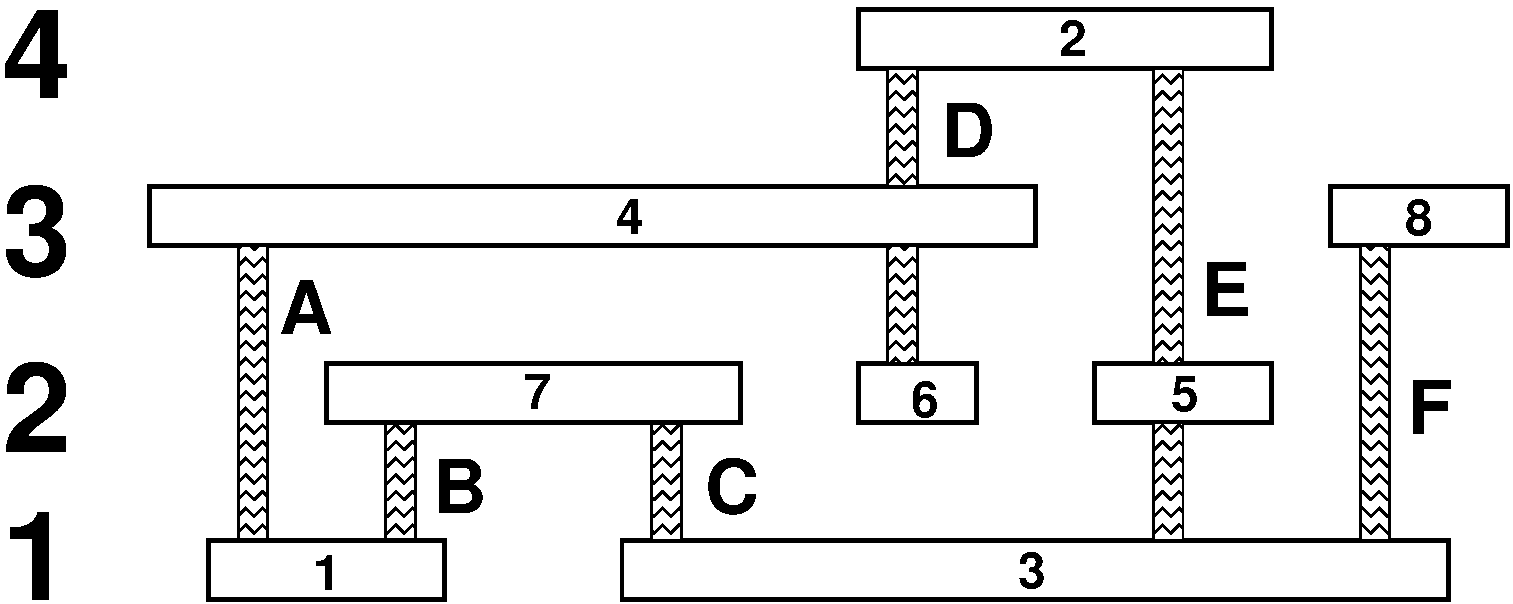
\includegraphics[width=11cm]{orient.pdf}
\end{minipage}
\vspace{0.5cm}
\;\\
\fe{Körningsexempel 1}\\
\begin{verbatim}
N ? 3
Omr 1, vån ? 2
Omr 1, tr  ? A
Omr 2, vån ? 4
Omr 2, tr  ? B
Omr 3, vån ? 7
Omr 3, tr  ? AB

Svar: 11
\end{verbatim}
\columnbreak
%\vspace{8cm}
~\\
~\\
~\\
~\\
~\\
~\\
~\\
~\\
~\\

Figuren ovan: Genomskärning av byggnaden i exempel 2. De stora siffrorna visar våningsnummer, de små numreringen av områdena. En möjlig kortaste väg genom hela banan är:\\
%(1) AAD (2) EEE (3) CBAA (4) DEE (5) EEDD (6) DAAB (7) CFF (8)\\
AAD -- EEE -- CBAA -- DEE -- EEDD -- DAAB -- CFF \\
Notera att kontrollerna måste tas i ordning. %, så även om område 4 besökts redan på väg till område 2 så måste det besökas igen efter område 3.
\end{multicols*}


%På sin väg mellan två områden kan orienteraren naturligtvis behöva passera andra områden, men dessa måste ändå uppsökas på sin riktiga tid (eftersom orienteringskontroller alltid måste tas i en viss ordning).


\newpage
\specialsection*{Uppgift 4 -- Dragkamp}

Under en idrottslektion vill läraren dela in alla elever i två lag för att tävla i dragkamp.
För att göra dragkampen intressant bör lagen vara exakt lika stora, samt exakt lika starka.
Läraren har på förhand uppskattat varje elevs styrka till ett tal mellan $1$ och $4$.

Givet hur många elever av varje styrketal som är med på lektionen, kan du berätta hur läraren ska dela upp lagen?
Det är garanterat att elevernas styrkor är valda så att detta alltid är möjligt.

Programmet ska läsa in de fyra heltalen $s_1, s_2, s_3, s_4$ ($0 \le s_i \le 10^{7}$), där $s_i$ är antalet elever som har styrkan $i$. 

%Om det inte är möjligt att dela in de två lagen ska programmet skriva ut en rad med texten ''\texttt{nej}''.
%Annars, skriv ut 
Programmet ska skriva ut en rad med fyra heltal $a_1, a_2, a_3, a_4$, där $a_i$ är antalet elever med styrkan $i$ som ska vara med i det ena dragkampslaget.

\fe{Poängsättning:}\\
För testfall värda $1$ poäng gäller $s_i \le 300$.\\
För testfall värda ytterligare $1$ poäng gäller $s_i \le 3000$.\\
För testfall värda $1$ poäng gäller att $s_4=0$, alltså att ingen elev har styrka $4$.\\
För de sista $2$ poängen gäller inga av dessa begränsningar. \\
%Testfallen är indelade i grupper och för att få poäng för en grupp så måste du klara alla testfall i gruppen.


\fe{Körningsexempel 1}\\
\begin{verbatim}
Antal ettor ? 1
Antal tvåor ? 1
Antal treor ? 1
Antal fyror ? 1

Svar: 1 0 0 1
\end{verbatim}

\fe{Körningsexempel 2}\\
\begin{verbatim}
Antal ettor ? 2
Antal tvåor ? 4
Antal treor ? 6
Antal fyror ? 8

Svar: 1 2 3 4
\end{verbatim}

%\fe{Förklaring:}


\newpage
\specialsection*{Uppgift 5 -- Sista moroten}

Det är frustrerande för Tor och hans mor att det ibland blir en morot kvar (se uppgift 1, \emph{Morötter}).
Istället för att dela den föreslår Tor att slå tärning om vem som ska få moroten.
Han tar fram $N$ stycken $M$-sidiga tärningar, vars sidor är numrerade från $1$ till $M$ och har exakt lika stor sannolikhet att rullas.
Han låter nu sin mor välja $K$ stycken tal, och om talen på tärningarna summerar till ett av de talen vinner hon, annars vinner Tor.
Mor vill nu ha din hjälp att skriva ett program för att avgöra hennes chans att vinna om hon väljer sina utfall optimalt.


%Katastrof! Joshua och Olle vill ha en kaka, men det finns bara en kvar i burken. Istället för att dela den på två föreslår Joshua att slå tärning om vem som ska få kakan.
%Han tar fram $N$ stycken $M$-sidiga tärningar, vars sidor är numrerade från $1$ till $M$. Tack vare att Joshua lärt sig lite geometri har han bevisat att alla sidor är lika sannolika att rullas.
%Han låter Olle välja $K$ stycken tal, och om talen på tärningarna summerar till ett av de talen vinner Olle, annars vinner Joshua.
%Olle vill nu ha din hjälp att skriva ett program för att avgöra hans chans att vinna om han väljer sina utfall optimalt.


%\section*{Indata}
%Den första raden innehåller de tre heltalen $N, M, K$ ($1 \le N \le 20, 1 \le M, K \le 10000$), antalet tärningar, hur många sidor vardera tärning har och hur många utfall Olle får välja.

Programmet ska läsa in de tre heltalen $N, M, K$ ($1 \le N \le 20$, $1 \le M \le 10000$, $1 \le K < N \cdot M$), antalet tärningar, hur många sidor vardera tärning har och hur många utfall mor får välja.

Programmet ska skriva ut ett decimaltal -- den största sannolikheten mor kan ha att vinna om hon väljer sina utfall rätt. 
Svaret kommer accepteras om det har ett relativt fel om högst $10^{-5}$.

\fe{Poängsättning:}\\
De fem testfallen som vardera ger $1$ poäng har följande begränsningar utöver de som redan nämnts:
\begin{enumerate}
\item  $\;\;\;\;N=2, M \le 100 $    
\item  $\;\;\;\;N \le 6,  M \le 6 $ 
\item  $\;\;\;\;N \le 50, M \le 4 $   
\item  $\;\;\;\;N \le 40, M \le 40 $   
\item  $\;\;\;\;N \le 20, M \le 5000 $   
\end{enumerate}

\fe{Körningsexempel 1}
\begin{verbatim}
Antal tärningar N ? 2
Antal sidor M ? 6 
Antal utfall K ? 2

Svar: 0.30555556
\end{verbatim}

\fe{Körningsexempel 2}
\begin{verbatim}
Antal tärningar N ? 3
Antal sidor M ? 7
Antal utfall K ? 4

Svar: 0.41399417
\end{verbatim}

\fe{Körningsexempel 3}
\begin{verbatim}
Antal tärningar N ? 20
Antal sidor M ? 2189
Antal utfall K ? 2734

Svar: 0.36902844
\end{verbatim}

\end{document}
